\chapter{3D-Stereokalibrierung und Szenenrekonstruktion mit reellen Daten und Kameras unterschiedlicher Auflösung}

\section{Ergebnisse einer Stereoanalyse mit Kameras unterschiedlicher Auflösung}

\begin{figure}[!htb]
	\minipage{0.48\textwidth}
	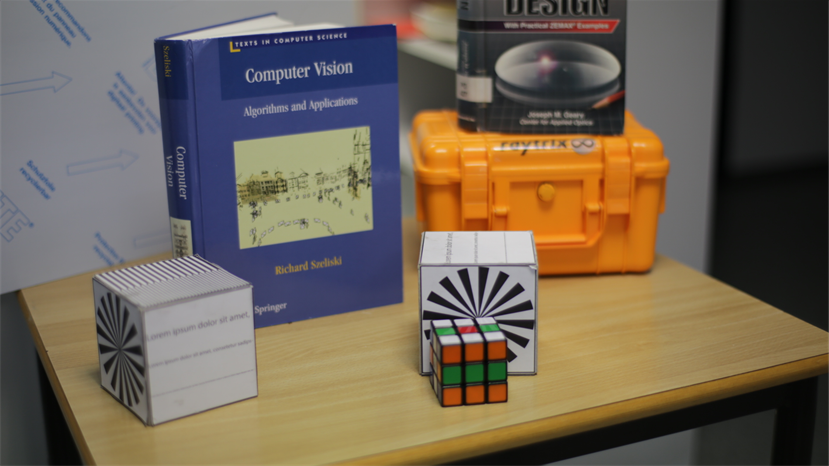
\includegraphics[width=\linewidth]{images/2Cameras2ResolutionsLeft.png}
	\caption{Canon 6D mit einer Auflösung von 1920 $\times$ 1080 und einem Seitenverältnis von 16:9}
	\label{fig:awesome_image1}
	\endminipage\hfill
	\minipage{0.48\textwidth}
	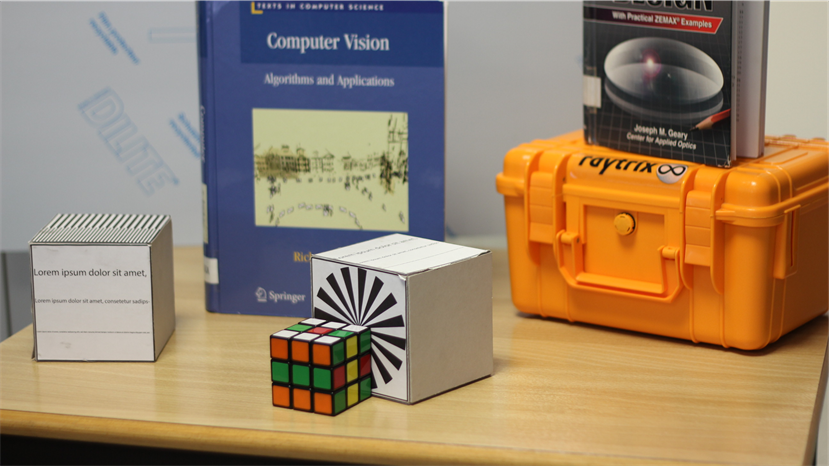
\includegraphics[width=\linewidth]{images/2Cameras2ResolutionsRight.png}
	\caption{Canon 6D mit einer Auflösung von 2.592 $\times$ 1.456 und einem Seitenverältnis von 16:9}
	\label{fig:awesome_image2}
	\endminipage\hfill
\end{figure}

\begin{figure}[!htb]
	\minipage{0.48\textwidth}
	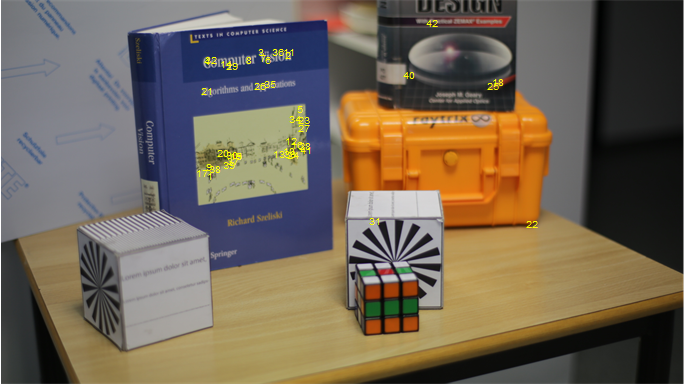
\includegraphics[width=\linewidth]{images/2Cameras2ResolutionsSURFLeft.png}
%	\caption{$C$ und $C'$ haben die selbe Auflösung eingestellt}
	\label{fig:awesome_image1}
	\endminipage\hfill
	\minipage{0.48\textwidth}
	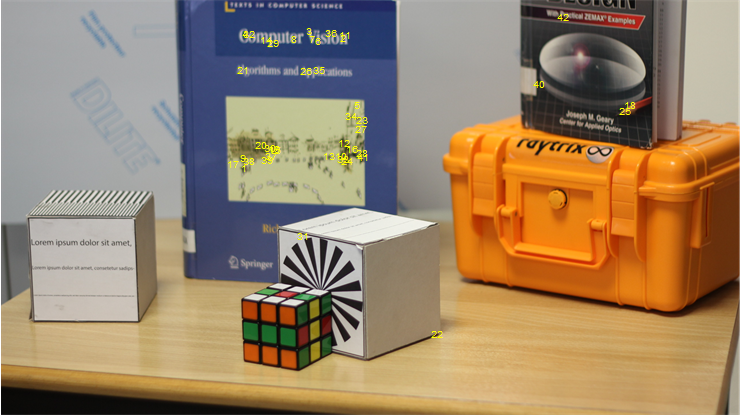
\includegraphics[width=\linewidth]{images/2Cameras2ResolutionsSURFRight.png}
%	\caption{$C$ und $C'$ haben unterschiedliche Auflösungen eingestellt}
	\label{fig:awesome_image2}
	\endminipage\hfill
	\caption{Die vom \textit{SURF}-Algorithmus gefundenen korrespondierenden Punkte sind durch die eine gelbe Numerierung gekennzeichnet}
\end{figure}


